% Thesis Figure 6.3: the two partner detection mechanisms, redrawn after D7.2 Figures 15
% and 16 (p. 16); the originals stay in ../sparta/report-originals/.
% (a) Prediction similarity, D7.2 Section 2.3.2.3.3: an external layer records user, image,
% prediction (class and probability), minimum distance to all previous images, prediction
% alarm and distance alarm; the history yields an alarm, and a suspicious query receives
% the opposite class.
% (b) Model's behaviour, D7.2 Section 2.3.2.3.4: nine statistics per hidden layer over 19
% layers give 171 features; after standardisation and selection, the detector is one SVC
% per class predicted by the original model.
% The response returns h XOR d, the label reversal D7.6 p. 28 applies in the benchmark.
% Symbols follow Chapter 6: d_t = d(x_t, H_{t-1}) in the text, z(x) from Equation
% eq:advml:activation-features, the response from Equation eq:advml:reversal.
% Colours as in Figure 6.2: filled blue is the external layer added by the defence, the
% blue outline the original classifier, white boxes data and signals.
% lmodern is loaded before the shared style so that math scales to the small sizes used
% here; the style then sets the text face to TeX Gyre Heros as in the other figures.
% Geometry is in millimetres with y pointing down; 140 mm fits the text block at 1:1.
\documentclass[border=1pt]{standalone}
\usepackage{lmodern}
\usepackage{amssymb}
% Shared typography and palette for the three corrected SWaT context figures.
% Geometry is in millimetres; 140 mm fits the thesis text block at native scale.
\usepackage[T1]{fontenc}
\usepackage{tgheros}
\renewcommand{\familydefault}{\sfdefault}
\usepackage{tikz}
\usetikzlibrary{calc,patterns}
\definecolor{swatblue}{HTML}{0065BD}
\definecolor{swatlight}{HTML}{98C6EA}
\definecolor{swatgrey}{HTML}{666666}
\tikzset{every node/.style={font=\fontsize{8}{10}\selectfont},
  panel/.style={draw=black!30,fill=white,line width=0.4pt},
  stage/.style={draw=swatblue,fill=swatblue,text=white,align=center,
    minimum height=10mm,text width=19mm,inner sep=0.5mm},
  smalllabel/.style={font=\fontsize{7}{8.5}\selectfont,text=swatgrey}}

\usetikzlibrary{arrows.meta}
\newcommand{\fT}{\fontsize{7.5}{9}\selectfont\bfseries}
\newcommand{\fH}{\fontsize{7}{8.4}\selectfont\bfseries}
\newcommand{\fB}{\fontsize{7}{8.4}\selectfont\mdseries}
\newcommand{\fS}{\fontsize{6.5}{7.8}\selectfont\mdseries}
\newcommand{\fX}{\fontsize{6}{7.2}\selectfont\mdseries}
\begin{document}
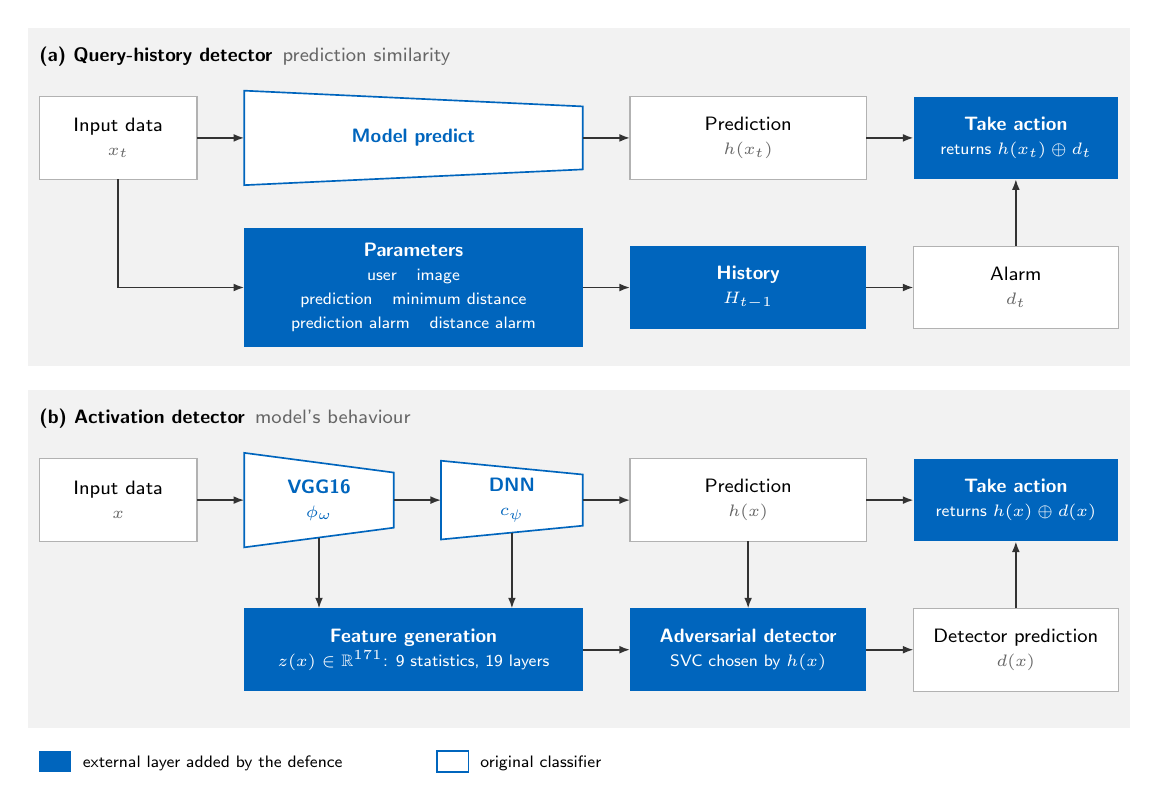
\begin{tikzpicture}[x=1mm,y=-1mm,
    txt/.style={inner sep=0pt,outer sep=0pt},
    ml/.style={txt,align=center,font=\fontsize{6}{7.2}\selectfont},
    op/.style={draw=black!30,fill=white,line width=0.4pt},
    netout/.style={draw=swatblue,fill=white,line width=0.6pt},
    lnk/.style={draw=black!80,line width=0.6pt},
    arr/.style={lnk,-{Latex[length=1.35mm,width=1mm]}}]
  \path[use as bounding box] (0,0) rectangle (140,96);

  % (a) Query-history detector: classifier lane at y = 14, detector lane at y = 33
  \fill[black!5] (0,0) rectangle (140,43);
  \node[txt,anchor=base west] at (1.5,4.3)
    {\fT (a) Query-history detector\hspace{1.3mm}{\fB\color{swatgrey}prediction similarity}};
  \draw[op] (1.5,8.75) rectangle (21.5,19.25);
  \node[ml] at (11.5,14) {{\fB Input data}\\[0.5mm]{\fX\color{swatgrey}$x_t$}};
  \draw[netout] (27.5,8) -- (70.5,10) -- (70.5,18) -- (27.5,20) -- cycle;
  \node[txt,text=swatblue] at (49,14) {\fH Model predict};
  \draw[op] (76.5,8.75) rectangle (106.5,19.25);
  \node[ml] at (91.5,14) {{\fB Prediction}\\[0.5mm]{\fX\color{swatgrey}$h(x_t)$}};
  \fill[swatblue] (112.5,8.75) rectangle (138.5,19.25);
  \node[ml,text=white] at (125.5,14)
    {{\fH Take action}\\[0.5mm]{\fX returns $h(x_t)\oplus d_t$}};
  \fill[swatblue] (27.5,25.5) rectangle (70.5,40.5);
  \node[ml,text=white] at (49,33) {{\fH Parameters}\\[0.5mm]{\fX user\hspace{2.5mm}image}\\[0.5mm]%
    {\fX prediction\hspace{2.5mm}minimum distance}\\[0.5mm]%
    {\fX prediction alarm\hspace{2.5mm}distance alarm}};
  \fill[swatblue] (76.5,27.75) rectangle (106.5,38.25);
  \node[ml,text=white] at (91.5,33) {{\fH History}\\[0.5mm]{\fX$H_{t-1}$}};
  \draw[op] (112.5,27.75) rectangle (138.5,38.25);
  \node[ml] at (125.5,33) {{\fB Alarm}\\[0.5mm]{\fX\color{swatgrey}$d_t$}};
  \draw[arr] (21.5,14) -- (27.5,14);
  \draw[arr] (70.5,14) -- (76.5,14);
  \draw[arr] (106.5,14) -- (112.5,14);
  \draw[arr] (11.5,19.25) -- (11.5,33) -- (27.5,33);
  \draw[arr] (70.5,33) -- (76.5,33);
  \draw[arr] (106.5,33) -- (112.5,33);
  \draw[arr] (125.5,27.75) -- (125.5,19.25);

  % (b) Activation detector: classifier lane at y = 60, detector lane at y = 79
  \fill[black!5] (0,46) rectangle (140,89);
  \node[txt,anchor=base west] at (1.5,50.3)
    {\fT (b) Activation detector\hspace{1.3mm}{\fB\color{swatgrey}model's behaviour}};
  \draw[op] (1.5,54.75) rectangle (21.5,65.25);
  \node[ml] at (11.5,60) {{\fB Input data}\\[0.5mm]{\fX\color{swatgrey}$x$}};
  \draw[netout] (27.5,54) -- (46.5,56.5) -- (46.5,63.5) -- (27.5,66) -- cycle;
  \node[ml,text=swatblue] at (37,60) {{\fH VGG16}\\[0.5mm]{\fX$\phi_\omega$}};
  \draw[netout] (52.5,55) -- (70.5,56.75) -- (70.5,63.25) -- (52.5,65) -- cycle;
  \node[ml,text=swatblue] at (61.5,60) {{\fH DNN}\\[0.5mm]{\fX$c_\psi$}};
  \draw[op] (76.5,54.75) rectangle (106.5,65.25);
  \node[ml] at (91.5,60) {{\fB Prediction}\\[0.5mm]{\fX\color{swatgrey}$h(x)$}};
  \fill[swatblue] (112.5,54.75) rectangle (138.5,65.25);
  \node[ml,text=white] at (125.5,60)
    {{\fH Take action}\\[0.5mm]{\fX returns $h(x)\oplus d(x)$}};
  \fill[swatblue] (27.5,73.75) rectangle (70.5,84.25);
  \node[ml,text=white] at (49,79)
    {{\fH Feature generation}\\[0.5mm]{\fX$z(x)\in\mathbb{R}^{171}$: 9 statistics, 19 layers}};
  \fill[swatblue] (76.5,73.75) rectangle (106.5,84.25);
  \node[ml,text=white] at (91.5,79) {{\fH Adversarial detector}\\[0.5mm]{\fX SVC chosen by $h(x)$}};
  \draw[op] (112.5,73.75) rectangle (138.5,84.25);
  \node[ml] at (125.5,79) {{\fB Detector prediction}\\[0.5mm]{\fX\color{swatgrey}$d(x)$}};
  \draw[arr] (21.5,60) -- (27.5,60);
  \draw[arr] (46.5,60) -- (52.5,60);
  \draw[arr] (70.5,60) -- (76.5,60);
  \draw[arr] (106.5,60) -- (112.5,60);
  % Activations of both networks feed the features; the prediction selects the SVC
  \draw[arr] (37,64.75) -- (37,73.75);
  \draw[arr] (61.5,64.125) -- (61.5,73.75);
  \draw[arr] (91.5,65.25) -- (91.5,73.75);
  \draw[arr] (70.5,79) -- (76.5,79);
  \draw[arr] (106.5,79) -- (112.5,79);
  \draw[arr] (125.5,73.75) -- (125.5,65.25);

  % Legend
  \fill[swatblue] (1.5,91.9) rectangle (5.5,94.5);
  \node[txt,anchor=base west] at (7,94) {\fS external layer added by the defence};
  \draw[netout] (52,91.9) rectangle (56,94.5);
  \node[txt,anchor=base west] at (57.5,94) {\fS original classifier};
\end{tikzpicture}
\end{document}
